\documentclass[11pt]{article}
\usepackage[margin=1in]{geometry}
\usepackage{amsmath,amssymb,amsthm}
\usepackage{enumitem}
\usepackage{booktabs}
\usepackage{tikz}
\usetikzlibrary{arrows.meta,positioning}
\usepackage{algorithm}
\usepackage{algpseudocode}
\usepackage{longtable}

\newtheorem{theorem}{Theorem}
\newtheorem{proposition}[theorem]{Proposition}
\newtheorem{corollary}[theorem]{Corollary}
\newtheorem{lemma}[theorem]{Lemma}
\theoremstyle{definition}
\newtheorem{definition}[theorem]{Definition}
\newtheorem{example}[theorem]{Example}
\theoremstyle{remark}
\newtheorem{remark}[theorem]{Remark}
\newtheorem{openproblem}[theorem]{Open problem}

\newcommand{\eps}{\tilde{\epsilon}}
\newcommand{\phist}{\tilde{\varphi}^*}
\newcommand{\Z}{\mathbb{Z}}
\newcommand{\N}{\mathbb{N}}

\title{Spoof Lehmer Factorizations:\\
Forest Structure, Plus-Seed Chains,\\
and a Closed-Form Finishing Algorithm}
\author{G.\ Molnar}
\date{\today~(Draft)}

\begin{document}
\maketitle

\begin{abstract}
We study spoof Lehmer factorizations through the lens of an
\emph{extension graph}~$\mathcal{G}_k$, building on Hasanalizade's
two-factor extension reduction and the Molnar--Singh framework.  Three
results characterize the global structure of $\mathcal{G}_k$:
(i)~positive-integer extensions arise exclusively from \emph{plus-seed}
states (those with $k\phist = \eps + 1$); (ii)~the descent formula
relating the evaluation of a Lehmer factorization to its descended
pair is independent of~$k$; and (iii)~$\mathcal{G}_k$ is a
\textbf{forest} for every $k \ge 2$.  We then develop the algorithmic
side: three closed-form finishing-feasibility identities (at
$s = r-1, r-2, r-3$) replace the deepest levels of bounds-propagation
with direct algebraic solves, completing the $r \le 7$ census ($107$
factorizations) in minutes where prior code stalled.  Tying the two
threads together, we prove a \emph{plus-seed chain extension theorem}
showing that every plus-seed initiates an infinite chain
$F^* \subset F^* \cdot (E + 2) \subset \cdots$, of which the Fermat
partial products are one chain and $(5, 5, 5, 43, 5377, \ldots)$ is the
first known sporadic chain.  A coprimality lemma yields a
\emph{plus-seed closedness theorem}: from any plus-seed of length $s$,
the length-$(s+2)$ Lehmer extensions number exactly $\tau(M)/2$ where
$M = E^2 + E - 1$.  This gives closed-form enumeration of two
canonical $r = 8$ subtrees (the length-8 extensions of Fermat-6 and
sporadic-6 plus-seeds), the first computational data at $r = 8$.
\end{abstract}


%=====================================================================
\section{Introduction}
%=====================================================================

Molnar and Singh~\cite{MS26} introduced the study of \emph{spoof Lehmer
factorizations}: multisets $F = \{x_1, \ldots, x_r\}$ of positive integers
satisfying
\begin{equation}\label{eq:lehmer}
  k\,\phist(F) = \eps(F) - 1,
  \qquad k \in \Z_{>0},
\end{equation}
where $\eps(F) = \prod x_i$ and $\phist(F) = \prod (x_i - 1)$.
Hasanalizade~\cite{H26} proved that if a factorization~$F$ satisfies the
auxiliary condition $k\,\phist(F) = \eps(F) + \alpha$ for
$\alpha \in \{-1, +1\}$, then the search for two-factor extensions
$F \cdot x \cdot y$ satisfying~\eqref{eq:lehmer} reduces to factoring a
single explicit integer (Equation~\eqref{eq:hasanalizade} below).

This paper investigates the global structure that the Hasanalizade
extension imposes on the solution set, develops a closed-form
finishing algorithm for enumeration, and uses both threads to study
the family structure that emerges.  The main contributions are:
\begin{enumerate}[label=(\roman*)]
  \item A proof that only $\alpha = +1$ seeds can produce extensions
    with positive factors (Theorem~\ref{thm:positive-only}).
  \item A closed-form descent criterion
    (Theorem~\ref{thm:descent-formula}) and the observation that it
    is \emph{independent of~$k$} (Corollary~\ref{cor:k-free}).
  \item A proof that the extension graph~$\mathcal{G}_k$ is a forest
    for every $k \ge 2$ (Theorem~\ref{thm:forest}).
  \item Three closed-form finishing-feasibility identities at
    $s = r - 1$, $r - 2$, $r - 3$
    (Propositions~\ref{prop:rm1}--\ref{prop:rm3}) that replace the
    deepest levels of bounds-propagation with direct algebraic solves.
  \item A complete computational census for $r \le 7$ across all
    valid $k$ (Theorem~\ref{thm:census}), comprising $107$
    factorizations.
  \item A plus-seed chain extension theorem
    (Theorem~\ref{thm:chain-existence}): every plus-seed initiates
    an infinite chain, of which the Fermat partial products are one
    instance and $(5, 5, 5, 43, 5377, \ldots)$ is the first known
    sporadic instance.
  \item A coprimality lemma
    (Lemma~\ref{lem:coprime}) and resulting plus-seed closedness
    theorem (Theorem~\ref{thm:plus-seed-closure}): the length-$(s+2)$
    Lehmer extensions of any length-$s$ plus-seed number exactly
    $\tau(M)/2$ for $M = E^2 + E - 1$.
  \item Closed-form enumeration of two canonical $r = 8$ subtrees,
    yielding the first concrete $r = 8$ data
    (Section~\ref{sec:r8-partial}).
\end{enumerate}


%=====================================================================
\section{Preliminaries}
%=====================================================================

We follow the notation of~\cite{MS26} and~\cite{H26}.  A \emph{spoof
factorization} is a finite multiset $F = x_1 \cdots x_r$ of positive
integers with $x_i \ge 2$, with \emph{spoof evaluation}
$\eps(F) = \prod x_i$ and \emph{spoof unitary totient}
$\phist(F) = \prod(x_i - 1)$.  We write $|F| = r$ for the number of
factors.  A factorization~$F$ with $|F| \ge 2$ is \emph{unitary $k$-Lehmer}
if~\eqref{eq:lehmer} holds.

\begin{definition}\label{def:seed}
A factorization~$F$ is an \emph{$\alpha$-seed} (with respect to~$k$) if
$k\,\phist(F) = \eps(F) + \alpha$, where $\alpha \in \{-1, +1\}$.  When
$\alpha = +1$, we call $F$ a \emph{plus-seed}.
\end{definition}

Hasanalizade's Theorem~3 in~\cite{H26} states that if~$F$ is an
$\alpha$-seed with $N = \eps(F)$, then $F \cdot x \cdot y$ is $k$-Lehmer
if and only if
\begin{equation}\label{eq:hasanalizade}
  (\alpha x - N - \alpha)(\alpha y - N - \alpha) = N^2 + \alpha N - \alpha.
\end{equation}

We also use the \emph{deficiency function} $g(F) = k\,\phist(F) - \eps(F)$,
which satisfies the recurrence
\begin{equation}\label{eq:recurrence}
  g(F \cdot a) = (a-1)\,g(F) - \eps(F), \qquad g(\emptyset) = k - 1.
\end{equation}
Lehmer factorizations correspond to $g = -1$, plus-seeds to $g = 1$.


%=====================================================================
\section{Only plus-seeds produce positive extensions}
%=====================================================================

\begin{theorem}\label{thm:positive-only}
Let $k \ge 2$ and let~$F$ be a $(-1)$-seed with $\eps(F) = N \ge 1$.  Then
Equation~\eqref{eq:hasanalizade} has no solutions with $x, y \ge 2$.
\end{theorem}

\begin{proof}
For $\alpha = -1$, Equation~\eqref{eq:hasanalizade} becomes
$(x + N - 1)(y + N - 1) = N^2 - N + 1$.  If $x, y \ge 2$ then the left
side is at least $(N+1)^2 = N^2 + 2N + 1 > N^2 - N + 1$ for all
$N \ge 1$.
\end{proof}


%=====================================================================
\section{The descent formula is $k$-independent}
%=====================================================================

\begin{definition}\label{def:descent}
Let~$G$ be a $k$-Lehmer factorization.  An unordered pair $\{a, b\}$ of
factors of~$G$ (counted with multiplicity) is a \emph{descended pair} if
$F = G \setminus \{a, b\}$ is a plus-seed from which~$G$ arises via
Equation~\eqref{eq:hasanalizade}.  We call~$G$ \emph{primitive} if
it admits no descended pair, and \emph{derived} otherwise.
\end{definition}

\begin{theorem}[Descent formula]\label{thm:descent-formula}
Let $k \ge 2$ and let~$G$ be a $k$-Lehmer factorization with
$\eps(G) = N$.  An unordered pair $\{a, b\}$ of factors of~$G$ is a
descended pair if and only if
\begin{equation}\label{eq:descent}
  N(a + b - 1) = ab\bigl((a-1)(b-1) + 1\bigr).
\end{equation}
\end{theorem}

\begin{proof}
The sub-factorization $F = G \setminus \{a, b\}$ has
$\eps(F) = N/(ab)$ and $\phist(F) = \phist(G)/\bigl((a-1)(b-1)\bigr)$.
Since~$G$ is $k$-Lehmer and~$F$ is a plus-seed:
\[
  k\,\phist(F) = \frac{k\,\phist(G)}{(a-1)(b-1)} = \frac{N-1}{(a-1)(b-1)},
  \qquad
  k\,\phist(F) = \frac{N}{ab} + 1.
\]
Equating:
\begin{equation}\label{eq:k-cancels}
  \frac{N - 1}{(a-1)(b-1)} = \frac{N}{ab} + 1.
\end{equation}
Clearing denominators: $(N-1)\,ab = N(a-1)(b-1) + ab(a-1)(b-1)$.
Expanding $N(a-1)(b-1) = N(ab - a - b + 1)$ and collecting:
\[
  N(a + b - 1) = ab\bigl(ab - a - b + 2\bigr) = ab\bigl((a-1)(b-1)+1\bigr).
  \qedhere
\]
\end{proof}

\begin{corollary}[$k$-independence]\label{cor:k-free}
The descent formula~\eqref{eq:descent} is independent of~$k$.
Equivalently, whether a pair $\{a,b\}$ can be a descended pair is
determined entirely by the multiset of factors and the evaluation~$N$, not
by the value of~$k$.
\end{corollary}

\begin{proof}
Equation~\eqref{eq:k-cancels} shows that $k$ cancels in the passage from
the $k$-Lehmer and plus-seed conditions to~\eqref{eq:descent}.
\end{proof}

\begin{remark}
The $k$-independence is perhaps surprising: the Lehmer condition $k\phist =
\eps - 1$ and the plus-seed condition $k\phist = \eps + 1$ both involve~$k$
explicitly, but dividing the first by the second at the level of a
descended pair absorbs~$k$ into the relationship between $\{a,b\}$ and
the remaining factors.
\end{remark}


%=====================================================================
\section{The extension graph is a forest}\label{sec:forest}
%=====================================================================

\begin{definition}
The \emph{extension graph} $\mathcal{G}_k$ is a directed graph whose
vertices are the $k$-Lehmer factorizations with factors $\ge 2$.  There is
an edge $G \to F$ whenever~$F = G \setminus \{a, b\}$ for some descended
pair $\{a, b\}$.
\end{definition}

\begin{theorem}[Forest theorem]\label{thm:forest}
For every $k \ge 2$, the extension graph~$\mathcal{G}_k$ is a forest:
every $k$-Lehmer factorization with factors $\ge 2$ admits at most one
descended pair.
\end{theorem}

By Corollary~\ref{cor:k-free}, the descent formula~\eqref{eq:descent} is
$k$-independent, so the entire proof reduces to showing that no single
multiset~$G$ with $\eps(G) = N$ can have two distinct unordered pairs
satisfying~\eqref{eq:descent} with an appropriate divisibility and
positivity structure.  The proof uses three lemmas, covering the three
possible cases for the intersection of two descended pairs.

\begin{lemma}[Disjoint case]\label{lem:disjoint}
Let~$G$ be a $k$-Lehmer factorization.  Then~$G$ cannot admit two
descended pairs $\{a,b\}$ and $\{c,d\}$ with
$\{a,b\} \cap \{c,d\} = \emptyset$.
\end{lemma}

\begin{proof}
Write $G = \{a, b, c, d\} \cup E$ with $\eps(E) = Q$ (where $Q = 1$ if
$E = \emptyset$), so $N = abcdQ$.  Applying the descent
formula~\eqref{eq:descent} to each pair and dividing by~$ab$ and~$cd$
respectively:
\begin{align}
  \label{eq:dj-I}
  cdQ\,(a+b-1) &= (a\!-\!1)(b\!-\!1)+1, \\
  \label{eq:dj-II}
  abQ\,(c+d-1) &= (c\!-\!1)(d\!-\!1)+1.
\end{align}
Since $(a-1)(b-1) + 1 \le ab$ for $a,b \ge 2$ (with strict inequality
unless one of $a, b$ equals~$1$), multiplying gives
\[
  a^2b^2c^2d^2\,Q^2\,(a\!+\!b\!-\!1)(c\!+\!d\!-\!1) \le a^2b^2c^2d^2,
\]
whence $Q^2(a+b-1)(c+d-1) \le 1$.  Since $a+b-1 \ge 3$ and $c+d-1 \ge 3$,
we get $Q^2 \le 1/9 < 1$, so $Q < 1$.

If $E \ne \emptyset$ then $Q \ge 2$, a contradiction.  If
$E = \emptyset$ then $Q = 1$ and~\eqref{eq:dj-I}--\eqref{eq:dj-II} become
$cd(a+b-1) = (a-1)(b-1)+1$ and $ab(c+d-1) = (c-1)(d-1)+1$.  The first
gives $cd < ab/(a+b-1) \le ab/3$; the second gives $ab < cd/(c+d-1) \le
cd/3$.  Together: $cd < ab/3 < cd/9$, which is absurd.
\end{proof}


\begin{lemma}[Overlapping case]\label{lem:overlap}
Let~$G$ be a $k$-Lehmer factorization.  Then~$G$ cannot admit two
descended pairs $\{a,b\}$ and $\{b,d\}$ sharing one element, where
$a \ne d$.
\end{lemma}

\begin{proof}
Write $G = \{a, b, d\} \cup E$ with $\eps(E) = Q$, so $N = abdQ$.  The
descent formula for each pair gives
\begin{align}
  \label{eq:ov-I}
  dQ\,(a+b-1) &= (a\!-\!1)(b\!-\!1)+1, \\
  \label{eq:ov-II}
  aQ\,(b+d-1) &= (b\!-\!1)(d\!-\!1)+1.
\end{align}
Bounding: $dQ \le ab/(a+b-1)$ and $aQ \le bd/(b+d-1)$.  Multiplying:
\[
  adQ^2 \le \frac{ab^2d}{(a+b-1)(b+d-1)},
  \qquad\text{so}\qquad
  Q^2 \le \frac{b^2}{(a+b-1)(b+d-1)}.
\]
We claim $(a+b-1)(b+d-1) > b^2$ for all $a,b,d \ge 2$.  Expanding:
\begin{align*}
  (a+b-1)(b+d-1) - b^2
    &= a(b+d-1) + b(d-2) + (1-d) \\
    &\ge 2(b+d-1) + 0 + (1-d)
    = 2b+d-1
    \ge 3.
\end{align*}
Therefore $Q^2 < 1$, which is impossible if $E \ne \emptyset$ (since then
$Q \ge 2$).

If $E = \emptyset$, then $|G| = 3$, $Q = 1$, and~$G = \{a,b,d\}$.  The
seed of $\{a,b\}$ is the single-element factorization~$(d)$, and the
plus-seed condition $k(d-1) = d + 1$ gives $d = (k+1)/(k-1)$.  By
symmetry, the seed of $\{b,d\}$ forces $a = (k+1)/(k-1)$.  We consider
three sub-cases:
\begin{itemize}
  \item $k = 2$: $d = a = 3$, $G = \{3, b, 3\}$, $N = 9b$.  The Lehmer
    condition $2 \cdot 2(b-1) \cdot 2 = 9b - 1$ gives $8b - 8 = 9b - 1$,
    hence $b = -7$.
  \item $k = 3$: $d = a = 2$, $G = \{2, b, 2\}$, $N = 4b$.  The Lehmer
    condition $3 \cdot 1 \cdot (b-1) \cdot 1 = 4b - 1$ gives
    $3b - 3 = 4b - 1$, hence $b = -2$.
  \item $k \ge 4$: $(k+1)/(k-1)$ is not an integer (since $k - 1 \ge 3$
    and $\gcd(k-1, k+1) \mid 2$), so no single-element plus-seed exists
    and the $|G| = 3$ case is vacuous.
\end{itemize}
In all cases, no valid factorization arises.
\end{proof}


\begin{lemma}[Repeated-element case]\label{lem:repeated}
Let~$G$ be a $k$-Lehmer factorization.  Then~$G$ cannot admit descended
pairs $\{v,v\}$ and $\{v,w\}$ with $w \ne v$, where $v$ appears with
multiplicity at least two in~$G$.
\end{lemma}

\begin{proof}
Write $G = \{v, v, w\} \cup E$ with $\eps(E) = Q$, so $N = v^2 wQ$.  The
descent formula for the pair~$\{v,v\}$ gives, after dividing by~$v^2$:
\begin{equation}\label{eq:rep-key}
  wQ(2v-1) = (v-1)^2 + 1.
\end{equation}
The left side is a positive multiple of $2v - 1$, so
$(2v-1) \mid \bigl((v-1)^2 + 1\bigr)$.  We compute modulo $2v-1$: since
$2(v-1) \equiv -1 \pmod{2v-1}$,
\[
  4\bigl((v-1)^2 + 1\bigr) = (2v-2)^2 + 4 \equiv 1 + 4 = 5 \pmod{2v-1}.
\]
As $\gcd(4, 2v-1) = 1$, we conclude $(2v-1) \mid 5$, giving
$2v - 1 \in \{1, 5\}$ and $v \in \{1, 3\}$.

For $v = 3$: Equation~\eqref{eq:rep-key} gives $5wQ = 5$, so $wQ = 1$,
forcing $w = 1$ and $Q = 1$.  But factors must be $\ge 2$.

For $v = 1$: factors must be $\ge 2$.

Neither case yields a valid factorization.
\end{proof}


\begin{proof}[Proof of Theorem~\ref{thm:forest}]
Let~$G$ be a $k$-Lehmer factorization with factors $\ge 2$, and suppose
for contradiction that $\{a,b\}$ and $\{c,d\}$ are two distinct descended
pairs.  There are three cases:
\begin{itemize}
  \item $\{a,b\} \cap \{c,d\} = \emptyset$: impossible by
    Lemma~\ref{lem:disjoint}.
  \item $|\{a,b\} \cap \{c,d\}| = 1$ with distinct values: after
    relabeling, $\{a,b\}$ and $\{b,d\}$ with $a \ne d$, impossible by
    Lemma~\ref{lem:overlap}.
  \item $|\{a,b\} \cap \{c,d\}| = 1$ with a repeated element: $\{v,v\}$
    and $\{v,w\}$, impossible by Lemma~\ref{lem:repeated}.
\end{itemize}
The only remaining possibility $\{a,b\} = \{c,d\}$ contradicts the
assumption that the pairs are distinct.
\end{proof}

\begin{corollary}\label{cor:unique-seed}
For any $k \ge 2$, every derived $k$-Lehmer factorization is produced
by a unique plus-seed.
\end{corollary}


%=====================================================================
\section{Finishing-feasibility identities}\label{sec:finishing}
%=====================================================================

The forest structure (Section~\ref{sec:forest},
Theorem~\ref{thm:forest}) characterizes which factorizations descend
from which seeds, but explicit enumeration still requires a search
procedure.  We now develop three closed-form identities that replace
the deepest levels of the bounds-propagation algorithm of~\cite{MS26}
with direct algebraic solves.  These are the algorithmic backbone of
the census in Section~\ref{sec:census}.

\subsection{Finishing-feasibility at $s = r - 1$}

Let $F_0 = (x_1, \ldots, x_{r-1})$ be a partial factorization with
$\eps(F_0) = E$ and $\phist(F_0) = P$.  A single factor~$x_r$ completes
$F_0$ to a $k$-Lehmer factorization iff
$k P (x_r - 1) = E x_r - 1$.  Solving:
\begin{equation}\label{eq:r-1-finish}
  x_r \;=\; \frac{kP - 1}{kP - E}.
\end{equation}

\begin{proposition}[$s = r - 1$ finishing-feasibility]\label{prop:rm1}
A partial factorization $F_0$ of length $r - 1$ extends to a $k$-Lehmer
factorization if and only if $kP - E > 0$, $kP - E$ divides $kP - 1$,
and the quotient $x_r = (kP - 1)/(kP - E)$ satisfies $x_r \ge x_{r-1}$
and the appropriate parity condition.  The extension, when it exists,
is unique.
\end{proposition}

\begin{proof}
Let $x_r$ extend $F_0$ to a $k$-Lehmer factorization.  Then
$kP(x_r - 1) = E x_r - 1$, rearranging to $(kP - E) x_r = kP - 1$.
If $kP - E \le 0$, the left side is non-positive for $x_r \ge 1$ and
the right side is positive, a contradiction.  Otherwise $x_r = (kP -
1)/(kP - E)$ is forced, and integrality requires $kP - E$ to divide
$kP - 1$.
\end{proof}

\subsection{Finishing-feasibility at $s = r - 2$}

Let $F_0 = (x_1, \ldots, x_{r-2})$ with $\eps(F_0) = E$ and
$\phist(F_0) = P$.  We seek a pair $(a, b)$ with $a \le b$ and
$a \ge x_{r-2}$ completing $F_0$ to a $k$-Lehmer factorization.  The
defining equation expands to $kP(a - 1)(b - 1) = Eab - 1$, which
rearranges to $(kP - E)\,ab - kP(a + b) + (kP + 1) = 0$.  Write
$A = kP - E$ and $B = kP$.  Multiplying by $A$ and completing the
product on $a$ and $b$ yields
\begin{equation}\label{eq:finish}
  (A a - B)(A b - B) \;=\; B E - A.
\end{equation}

\begin{proposition}[$s = r - 2$ finishing-feasibility]\label{prop:rm2}
Let $F_0$ be a partial factorization of length $r - 2$, with $A = kP - E$
and $B = kP$.  A pair $(a, b)$ with $a \le b$ and $a \ge x_{r-2}$ extends
$F_0$ to a $k$-Lehmer factorization if and only if $A > 0$ and there is
a divisor pair $(d_1, d_2)$ of $BE - A$ with $d_1 \le d_2$ such that
\[
  a = \frac{d_1 + B}{A},
  \qquad
  b = \frac{d_2 + B}{A},
\]
are integers satisfying $x_{r-2} \le a \le b$ and the appropriate
parity and Lehmer-congruence conditions.
\end{proposition}

\begin{remark}[Relationship to the descent formula]
When $F_0$ is a plus-seed---i.e., $kP = E + 1$, so $A = 1$ and
$B = E + 1$---Equation~\eqref{eq:finish} becomes
$(a - E - 1)(b - E - 1) = (E + 1) E - 1 = E^2 + E - 1 = \Delta_+(E)$,
exactly the Hasanalizade descent equation~\eqref{eq:hasanalizade}.  The
$s = r - 2$ finishing-feasibility identity therefore subsumes the
Hasanalizade descent equation: the descent formula handles the case
$A = 1$; Proposition~\ref{prop:rm2} handles arbitrary $A \ge 1$.
\end{remark}

\subsection{Finishing-feasibility at $s = r - 3$}

Let $F_0 = (x_1, \ldots, x_{r-3})$.  We seek a triple $(a, b, c)$
with $x_{r-3} \le a \le b \le c$ completing $F_0$.  Substituting
$u = Aa - B$, $v = Ab - B$, $w = Ac - B$ in
$kP(a-1)(b-1)(c-1) = Eabc - 1$ and multiplying by $A^3$, we obtain
\begin{equation}\label{eq:3var-uvw}
  uvw \;-\; EB(u + v + w) \;=\; C_{F_0},
  \qquad
  C_{F_0} := A^2(E - 1) + E^2(3A + 2E).
\end{equation}
For each fixed $u \ge 1$, the remaining two-variable equation
multiplies through by $u$ and completes on $v, w$ to
\begin{equation}\label{eq:3var-fixed-u}
  (u v - EB)(u w - EB) \;=\; u \cdot C_{F_0} + u^2 EB + (EB)^2 =: M_u.
\end{equation}

\begin{proposition}[$s = r - 3$ finishing-feasibility]\label{prop:rm3}
A triple $(a, b, c)$ with $x_{r-3} \le a \le b \le c$ extends $F_0$
to a $k$-Lehmer factorization if and only if $A > 0$ and there exist
a positive integer $u$ and a divisor pair $(D_1, D_2)$ of $M_u$
satisfying $A \mid u + B$, $u \mid D_1 + EB$, $u \mid D_2 + EB$,
$A \mid v + B$, $A \mid w + B$ (where $v, w$ are computed from $D_1,
D_2$), $a \le b \le c$, and the parity/Lehmer-congruence conditions.
\end{proposition}

The outer loop over $u$ is bounded: since $v, w \ge u$, we have
$uvw \ge u^3$, so $u^3 \le 3 EB u + C_{F_0}$, giving
$u \le \sqrt{3 EB} + O(C_{F_0}^{1/3})$ to leading order.  For the
case of greatest interest---when $F_0$ is a plus-seed, where the
$s = r - 3$ identity governs $r = s + 3$ extensions---this bound
admits a clean closed form:

\begin{proposition}[$u_{\max}$ for plus-seeds]\label{prop:umax-plusseed}
Let $F^*$ be a $k = 2$ plus-seed with $\eps(F^*) = E$ (so $A = 1$,
$B = E + 1$, $C_{F^*} = 2E^3 + 3E^2 + E - 1$).  The
$s = r - 3$ finishing-feasibility identity at $F^*$ admits a positive
integer solution $u$ only in the range
\[
  1 \;\le\; u \;\le\; 2 E + 1.
\]
\end{proposition}

\begin{proof}
The constraint $u \le v \le w$ together with
Equation~\eqref{eq:3var-uvw} gives
$u^3 \le uvw = EB(u + v + w) + C_{F^*} \le 3 EB w + C_{F^*}$ when
$w \ge u$; combined with $u \le w$ this yields
$u^3 \le 3 EB u + C_{F^*}$.  At $u = 2(E + 1) = 2B$, the polynomial
identity
\[
  (2E + 2)^3 - 3 E (E+1)(2E + 2) - (2E^3 + 3E^2 + E - 1)
  \;=\; 9 E^2 + 17 E + 9
\]
is positive for all $E \ge 0$.  Hence $u^3 > 3 EB u + C_{F^*}$ at
$u = 2B$, so any productive $u$ must satisfy $u < 2B$, i.e.\
$u \le 2B - 1 = 2 E + 1$.
\end{proof}

\begin{remark}[Empirical gap]\label{rem:umax-empirical}
The bound $u \le 2E + 1$ matches the largest real root of $u^3 = 3EBu
+ C_{F^*}$ up to an $O(1)$ correction; it is essentially the best
obtainable from real-valued analysis.  Empirically, however,
productive $u$ tend to be substantially smaller.  For both length-$4$
plus-seeds appearing in our $r \le 7$ census---the Fermat-$4$ prefix
$(3, 5, 17, 257)$ with $E = 65535$ and the sporadic $(5, 5, 5, 43)$
with $E = 5375$---the maximum observed productive $u$ values are
$38557 \approx 0.588 \cdot E$ and $3373 \approx 0.628 \cdot E$
respectively, well below the provable bound $u \le 2E + 1$.  This
suggests the empirical conjecture $u_{\max}^2 \le EB$ for $k = 2$
plus-seeds (equivalently $u \le \sqrt{E(E+1)} \approx E$).
Spot-checks on the length-$5$ $k = 2$ plus-seeds confirm the pattern:
sampling $u$ at logarithmically spaced values in the range $(\sqrt{EB},
2E + 1]$ across three length-$5$ plus-seeds---namely $(5, 7, 7, 7, 133)$
with $E = 228\,095$, $(3, 9, 9, 23, 131)$ with $E = 732\,159$, and
$(5, 5, 5, 47, 453)$ with $E = 2\,661\,375$---produced zero
productive $u$ beyond $\sqrt{EB}$.  However, the divisor-density
heuristic does not produce
this bound: explicit computation of $\tau(M_u)/u$ at productive $u$
shows values as small as $\sim 10^{-4}$, so the existence of valid
divisors is not predicted by uniform-distribution arguments.  The
gap originates in the integrality requirement on $w = (D_2 + EB)/u$
together with the divisor structure of $M_u$ in the residue class
$-EB \pmod u$, which does not admit a closed-form bound.
\end{remark}

The pattern halts at $j = r - s = 3$: the substitution
$u_i = Ax_i - B$ reduces the defining equation to a $j$-variable
homogeneous-degree-$j$ problem; at $j = 2$ it is a hyperbola (exact
divisor solution); at $j = 3$ it is a cubic surface, planar only after
fixing one variable; at $j \ge 4$ even one-variable-fixed reductions
are non-planar.


%=====================================================================
\section{Algorithm}\label{sec:algorithm}
%=====================================================================

The sharpened bounds-propagation algorithm replaces the last three
levels of recursion with direct solves:

\begin{algorithm}[H]
\caption{Sharpened bounds propagation for $k$-Lehmer enumeration}
\label{alg:sharp}
\begin{algorithmic}[1]
\Procedure{Enumerate}{$F_0$, $k$, $r$}
\State $s \gets |F_0|$
\If{$s = r - 1$}
    \State solve~\eqref{eq:r-1-finish}; emit if integer and valid
\ElsIf{$s = r - 2$}
    \State factor $BE - A$; emit every divisor pair giving valid $(a, b)$
\ElsIf{$s = r - 3$}
    \For{each valid $u$ with $u^3 \le 3EBu + C_{F_0}$}
        \State factor $M_u$; emit every divisor pair giving valid $(b, c)$
    \EndFor
\Else
    \State apply bounds propagation as in~\cite{MS26}
    \For{each candidate $x_{s+1}$ not pruned by $L, U$ or Lehmer's
        congruence}
        \State \Call{Enumerate}{$F_0 \cup \{x_{s+1}\}$, $k$, $r$}
    \EndFor
\EndIf
\EndProcedure
\end{algorithmic}
\end{algorithm}

\begin{remark}[Cost structure]
The dominant cost is the integer factorizations at $s = r - 2$ and
$s = r - 3$.  For $r = 7$ at $k = 2$ odd, the integers to be factored
have at most~20 digits, and modern general-purpose factoring routines
(Pollard-rho plus ECM as implemented in SymPy~\cite{sympy}) factor
each in well under a millisecond.  A naive implementation using trial
division up to $\sqrt{M}$ is catastrophic here: $M$ reaches $\sim
10^{19}$, so the trial-division loop runs for several minutes per
prefix, where the factoring-based implementation finishes in
microseconds.
\end{remark}


%=====================================================================
\section{The complete $r \le 7$ census}\label{sec:census}
%=====================================================================

We implemented Algorithm~\ref{alg:sharp} and ran it for every
$(r, k)$ pair with $r \le 7$, $k \ge 2$, and factors odd and $\ge 3$.
The relevant $k$ range is finite: any $k$-Lehmer factorization with
minimum factor $a_{\min}$ and length $r$ satisfies
$k < (a_{\min} / (a_{\min} - 1))^r$, so for odd factors
$k \le \lfloor (3/2)^r \rfloor$.  At $r = 7$ this gives
$k \in \{2, 3, \ldots, 17\}$.

\begin{theorem}[$r \le 7$ census]\label{thm:census}
The complete set of $k$-Lehmer factorizations with $r \le 7$ and all
factors odd and $\ge 3$, across all valid $k \ge 2$, consists of
exactly~$107$ factorizations distributed as in
Table~\ref{tab:census-distribution}.  Only the values $k \in \{2, 4,
5, 8\}$ produce any such factorizations in this range.  Of the $103$
factorizations at $k = 2$, $50$ are Hasanalizade-descended (their
length-$(r-2)$ prefix is a plus-seed), $11$ are Lehmer companions of
plus-seeds (their length-$(r-1)$ prefix $P^*$ is a plus-seed and the
final factor is $\eps(P^*)$), $41$ are truly primitive (no plus-seed
parent of either kind), and one is the trivial $(3, 3)$.  The full
hierarchical listing appears in Appendix~\ref{app:full-census}.
\end{theorem}

\begin{table}[ht]
\centering
\caption{Distribution of odd $k$-Lehmer factorizations by length~$r$
and parameter~$k$, for $2 \le r \le 7$.  Columns for $k \notin
\{2,4,5,8\}$ are omitted (all zeros in this range).}
\label{tab:census-distribution}
\smallskip
\begin{tabular}{@{}rrrrrr@{}}
\toprule
$r$ & $k=2$ & $k=4$ & $k=5$ & $k=8$ & total \\
\midrule
2 & 1   & --- & --- & --- & 1 \\
3 & 1   & --- & --- & --- & 1 \\
4 & 1   & --- & 1   & --- & 2 \\
5 & 4   & --- & --- & --- & 4 \\
6 & 22  & 1   & --- & --- & 23 \\
7 & 74  & 1   & --- & 1   & 76 \\
\midrule
total & 103 & 2 & 1 & 1 & \textbf{107} \\
\bottomrule
\end{tabular}
\end{table}

\begin{proof}
By exhaustive enumeration using Algorithm~\ref{alg:sharp}.  The forest
property of Theorem~\ref{thm:forest} guarantees the parent-uniqueness
asserted for non-primitive factorizations.
\end{proof}

\subsection{Plus-seed chains observed in the census}

The forest theorem (Theorem~\ref{thm:forest}) guarantees every
non-primitive $k = 2$-Lehmer factorization in the census descends from
a unique plus-seed via Hasanalizade two-factor descent.  The
chain-extension theorem (Theorem~\ref{thm:chain-existence}) further
organizes the plus-seeds themselves into infinite chains rooted at
\emph{fresh} plus-seeds (those whose length-$(s-1)$ prefix is not a
plus-seed).  Combining these, each $k = 2$-Lehmer factorization is
attributable to a unique chain (or is truly primitive).

In the $r \le 7$ census we observe twelve such chains
(Table~\ref{tab:chains}): the Fermat chain rooted at $\emptyset$ and
eleven sporadic chains.  Six of the eleven sporadic chains have their
roots at length~$6$, detected here via inverting the parent
relationship from the $r = 7$ census without performing a length-$6$
plus-seed search.  The complete hierarchical listing of every
factorization in the census, organized under its parent plus-seed,
is given in Appendix~\ref{app:full-census}.

\begin{table}[ht]
\centering
\caption{Plus-seed chains observed in the $r \le 7$ census ($k = 2$,
odd).  Each chain is rooted at a \emph{fresh} plus-seed and continues
by $x = \eps + 2$ (Theorem~\ref{thm:chain-existence}).  The
\emph{member lengths} column lists the lengths at which the chain has
been observed in the census; the \emph{Lehmer descendants} column
gives the total number of $k = 2$-Lehmer factorizations descending
from any chain member, counting both Hasanalizade-descended and
Lehmer-companion children.}
\label{tab:chains}
\smallskip
\begin{tabular}{@{}lllr@{}}
\toprule
Chain & Root & Member lengths & Lehmer descendants \\
\midrule
Fermat & $\emptyset$ & $1, 2, 3, 4, 5$ & $24$ \\
sporadic & $(5, 5, 5, 43)$ & $4, 5$ & $10$ \\
sporadic & $(3, 5, 17, 353, 929)$ & $5$ & $5$ \\
sporadic & $(3, 9, 9, 23, 131)$ & $5$ & $2$ \\
sporadic & $(5, 5, 5, 47, 453)$ & $5$ & $9$ \\
sporadic & $(5, 7, 7, 7, 133)$ & $5$ & $5$ \\
sporadic & $(3, 5, 17, 257, 65729, 22318913)$ & $6$ & $1$ \\
sporadic & $(3, 5, 17, 365, 855, 7234467)$ & $6$ & $1$ \\
sporadic & $(3, 11, 11, 11, 677, 3659)$ & $6$ & $1$ \\
sporadic & $(5, 5, 5, 43, 5413, 786349)$ & $6$ & $1$ \\
sporadic & $(5, 5, 5, 53, 215, 158265)$ & $6$ & $1$ \\
sporadic & $(5, 7, 7, 13, 13, 619)$ & $6$ & $1$ \\
\bottomrule
\end{tabular}
\end{table}

\begin{remark}[Length-$6$ fresh plus-seeds without a length-$6$ search]
The six length-$6$ sporadic chain roots in Table~\ref{tab:chains} were
not found by an exhaustive length-$6$ plus-seed search (which is
prohibitively expensive at this length).  Each appears in our census
as the length-$(r - 1)$ prefix of an $r = 7$ Lehmer-companion
factorization $(P^*, \eps(P^*))$, where $P^*$ is the length-$6$
plus-seed.  Inverting this relationship across the census yields the
complete length-$6$ plus-seed inventory \emph{up to the limits of the
$r = 7$ census}---namely, every length-$6$ plus-seed whose Lehmer
companion has factors small enough to appear in the $r \le 7$ search
window.  Length-$6$ plus-seeds whose Lehmer companions exceed those
bounds (or which produce only length-$8$ or longer descendants) would
not be observed by this method, so the count of $11$ sporadic chains
is a lower bound on the true count of $r \le 7$-attributable chains.
\end{remark}

\subsection{Family structure at $r = 7$, $k = 2$}\label{subsec:families}

The $74$ factorizations at $r = 7$, $k = 2$ group by length-$5$ prefix
into families.  Of the $44$ length-$5$ prefixes appearing, exactly
four produce more than one length-$7$ completion, and \emph{all four
are plus-seeds}:
\begin{itemize}
  \item $(3, 5, 17, 257, 65537) = F^{(5)}$ (Fermat-$5$): $16$ completions.
  \item $(3, 5, 17, 353, 929)$ (sporadic): $4$ completions.
  \item $(5, 5, 5, 47, 453)$ (sporadic): $8$ completions.
  \item $(5, 7, 7, 7, 133)$ (sporadic): $4$ completions.
\end{itemize}
This corroborates the descent picture: completion multiplicity at
length $r - 2$ is governed by $\tau(M) / 2$ where
$M = E^2 + E - 1$, and multiplicity $\ge 2$ requires the prefix to be
a plus-seed (so that no divisor of $M$ is excluded by the
divisibility-mod-$A$ constraint).  At $r = 7$ with $k \ne 2$, exactly
two factorizations exist:
$(3, 3, 3, 9, 23, 131, 732159)$ at $k = 4$ and
$(3, 3, 3, 3, 5, 5, 89)$ at $k = 8$.


%=====================================================================
\section{Plus-seed chains}\label{sec:plus-seed-chains}
%=====================================================================

The plus-seeds in our census do not arise in isolation: they organize
themselves into infinite \emph{chains} via a canonical extension
operation.  The Fermat partial products form one such chain, but they
are not the only one.  This section develops the chain theory and
identifies its first sporadic instance.

\subsection{The canonical chain extension}

\begin{theorem}[Chain extension exists and is unique]\label{thm:chain-existence}
Let $F^*$ be a $k = 2$ plus-seed of length $s$ with $\eps(F^*) = E$
and $\phist(F^*) = P$.  Define $x := E + 2$.  Then $(F^*, x)$ is again
a $k = 2$ plus-seed.  Moreover, $x$ is the unique value of the next
factor for which this is the case.
\end{theorem}

\begin{proof}
For $(F^*, x)$ to be a plus-seed we require $2 P (x - 1) = E x + 1$,
i.e.\ $x(2P - E) = 2P + 1$.  Since $F^*$ is itself a plus-seed,
$2P - E = 1$ and $2P = E + 1$, so the equation simplifies to
$x = 2P + 1 = E + 2$.  Substituting $x = E + 2$ back, we have
$2P(x - 1) = (E+1)(E+1) = E^2 + 2E + 1 = E(E+2) + 1 = Ex + 1$, so
$(F^*, x)$ is indeed a plus-seed.
\end{proof}

\begin{lemma}[Chain extension is admissible]\label{lem:chain-admissible}
The next factor $x = E + 2$ in Theorem~\ref{thm:chain-existence} is
odd, satisfies $x > x_s$ (the last factor of $F^*$), and respects the
Lehmer congruence $x \not\equiv 1 \pmod{a}$ for every prior factor
$a$ in $F^*$.
\end{lemma}

\begin{proof}
\emph{Parity.}  Each factor of $F^*$ is odd (we restrict to the odd-spoof
setting throughout), so $E$ is odd and $E + 2$ is odd.

\emph{Ordering.}  $E = \prod_i x_i \ge x_s$ since each $x_i \ge 1$, and
in fact $E + 2 > x_s$ for any non-trivial $F^*$.

\emph{Lehmer congruence.}  $x - 1 = E + 1 = 2P$.  We need $a \nmid 2P$
for every prior factor $a$ in $F^*$.  Since $a$ is odd, this is
equivalent to $a \nmid P = \prod_j (x_j - 1)$.  By the Lehmer
congruence on $F^*$ itself, $a \nmid (x_j - 1)$ for all $j$ with
$x_j$ a factor of $F^*$ (taking $j$ to be the index of $a$ for the
trivial case, where $a \nmid (a-1)$ since $a \ge 3$).  Hence $a \nmid
P$.
\end{proof}

\begin{corollary}[Plus-seed chains are infinite]\label{cor:infinite-chain}
Every $k = 2$ plus-seed $F^*$ generates an infinite chain
\[
  F^* \;\subset\; F^* \cdot (E_0 + 2)
       \;\subset\; F^* \cdot (E_0 + 2,\, E_1 + 2)
       \;\subset\; \cdots
\]
of $k = 2$ plus-seeds, where $E_i$ is the value of $\eps$ at the
$i$-th step.
\end{corollary}

\subsection{The Fermat chain}

The Fermat partial products $F^{(s)} = \prod_{i=0}^{s-1}(2^{2^i}+1)$
form a linear chain of plus-seeds for $k = 2$, since the telescoping
identity
\[
  2\prod_{i=0}^{s-1} 2^{2^i}
    = 2^{2^s}
    = \prod_{i=0}^{s-1}(2^{2^i}+1) + 1
\]
gives $2\,\phist(F^{(s)}) = \eps(F^{(s)}) + 1$.  Each seed generates
Lehmer factorizations by factoring
$\Delta_+(2^{2^s}\!-\!1) = 2^{2^{s+1}} - 2^{2^s} - 1$.

This linear chain is precisely the chain that
Theorem~\ref{thm:chain-existence} produces from the root $(3)$:
$E^{(s)} = F_s - 2 = 2^{2^s} - 1$ (by telescoping), so
$E^{(s)} + 2 = 2^{2^s} + 1 = F_s$, and the canonical chain extension
yields the next Fermat number.

\begin{corollary}[Fermat chain identification]\label{cor:fermat-chain}
The chain extending $(3)$ via Theorem~\ref{thm:chain-existence} is the
sequence of Fermat partial products $F^{(s)} = (F_0, F_1, \ldots,
F_{s-1})$ for $s \ge 1$.
\end{corollary}

\subsection{The first sporadic chain}

The Fermat chain is not the only one.  Our $|F| \le 6$ census exhibits
a sporadic plus-seed at length~$4$:
\[
  S^{(4)} = (5, 5, 5, 43).
\]
By Theorem~\ref{thm:chain-existence} this extends to an infinite
chain
\[
  S^{(4)},\;
  S^{(5)} = (5, 5, 5, 43, 5377),\;
  S^{(6)} = (5, 5, 5, 43, 5377, 28901377),\;
  \ldots
\]
where $5375 + 2 = 5377$ and $5375 \cdot 5377 + 2 = 28901377$, etc.

The closed-form enumeration of length-$(s+2)$ extensions extends
from the Fermat case to every plus-seed:

\begin{lemma}[Coprimality lemma for plus-seeds]\label{lem:coprime}
For any $k = 2$ plus-seed $F^* = (x_1, \ldots, x_s)$ with $E =
\eps(F^*)$ and $M_{F^*} := E^2 + E - 1$, we have
$\gcd(M_{F^*}, x_i) = 1$ for every $i \in \{1, \ldots, s\}$.
\end{lemma}

\begin{proof}
$E = \prod_j x_j$ contains $x_i$ as a factor, so $E \equiv 0
\pmod{x_i}$.  Hence $M_{F^*} = E^2 + E - 1 \equiv -1 \pmod{x_i}$, and
$\gcd(M_{F^*}, x_i) \mid \gcd(-1, x_i) = 1$.
\end{proof}

\begin{theorem}[Plus-seed closedness at $r = s + 2$]\label{thm:plus-seed-closure}
Let $F^*$ be a $k = 2$ plus-seed of length $s$, with $E =
\eps(F^*)$ and $M_{F^*} = E^2 + E - 1$.  The $k = 2$-Lehmer
factorizations of length $s + 2$ extending $F^*$ are in bijection
with the divisors $d \le \sqrt{M_{F^*}}$ of $M_{F^*}$.  The
factorization corresponding to $d$ is
\[
  \bigl(F^*,\; d + (E + 1),\; M_{F^*}/d + (E + 1)\bigr),
\]
and the count is exactly $\tau(M_{F^*}) / 2$.
\end{theorem}

\begin{proof}
By the $s = r - 2$ finishing-feasibility identity
(Proposition~\ref{prop:rm2}) applied to $F^*$, the length-$(s+2)$ extensions
are in bijection with divisor pairs $(d, M_{F^*}/d)$ of $M_{F^*} =
B \cdot E - A = (E+1) \cdot E - 1$, with $a = d + B$ and $b =
M_{F^*}/d + B$ where $B = 2P = E + 1$ for any plus-seed.
Integrality follows from $A = 1$.  The Lehmer congruence (i.e.\
$x_i \nmid (a - 1)$ and $x_i \nmid (b - 1)$ for prior factors $x_i$)
holds because $a - 1 = d + E$ and $E \equiv 0 \pmod{x_i}$ implies
$a - 1 \equiv d \pmod{x_i}$, and by Lemma~\ref{lem:coprime},
$x_i \nmid d$ (since $d \mid M_{F^*}$ and $\gcd(M_{F^*}, x_i) = 1$).
The same applies to $b - 1$.  Parity holds because $E$ is a product
of odd factors, hence odd, so $E^2 + E$ is even and $M_{F^*} = E^2 +
E - 1$ is odd; all its divisors are odd.  The remaining ordering and
$a \mid b - 1$ checks are as in the Fermat
case (where the same argument was originally given for the Fermat
specialization).
\end{proof}

The theorem is verified empirically by the $r \le 7$ census: for each
of the eight $k = 2$ plus-seeds with length $\le 5$, the predicted
count $\tau(M_{F^*}) / 2$ matches the number of length-$(s+2)$
extensions found by exhaustive search:
\[
  \begin{array}{lll}
  (3, 5, 17, 257)              & \tau / 2 = 4  & \checkmark \\
  (5, 5, 5, 43)                & \tau / 2 = 8  & \checkmark \\
  (3, 5, 17, 257, 65537)        & \tau / 2 = 16 & \checkmark \\
  (3, 5, 17, 353, 929)          & \tau / 2 = 4  & \checkmark \\
  (3, 9, 9, 23, 131)            & \tau / 2 = 1  & \checkmark \\
  (5, 5, 5, 43, 5377)           & \tau / 2 = 1  & \checkmark \\
  (5, 5, 5, 47, 453)            & \tau / 2 = 8  & \checkmark \\
  (5, 7, 7, 7, 133)             & \tau / 2 = 4  & \checkmark
  \end{array}
\]

\subsection{Fresh plus-seeds and the chain forest}

We say a plus-seed of length $s \ge 2$ is a \emph{descendant} if its
length-$(s-1)$ prefix is itself a plus-seed; otherwise it is
\emph{fresh}.  By Theorem~\ref{thm:chain-existence}, each fresh
plus-seed initiates a unique infinite chain of descendant plus-seeds.
The set of all $k = 2$ plus-seeds, organized under the parent-child
relation $F^* \mapsto (F^*, E + 2)$, forms a disjoint union of
infinite linear chains rooted at the fresh plus-seeds.

\begin{table}[ht]
\centering
\caption{Plus-seed structure by length, $k = 2$, odd spoof.  Each
fresh plus-seed initiates an infinite descendant chain by
Corollary~\ref{cor:infinite-chain}; descendant plus-seeds are not
listed.}
\label{tab:plus-seeds-by-length}
\smallskip
\begin{tabular}{@{}rrrl@{}}
\toprule
length $s$ & total plus-seeds & fresh & fresh plus-seeds at this length \\
\midrule
$1$ & $1$ & $1$ & $(3)$ \\
$2$ & $1$ & $0$ & --- \\
$3$ & $1$ & $0$ & --- \\
$4$ & $2$ & $1$ & $(5, 5, 5, 43)$ \\
$5$ & $6$ & $4$ & $(3, 5, 17, 353, 929)$,~ $(3, 9, 9, 23, 131)$, \\
    &     &     & $(5, 5, 5, 47, 453)$,~ $(5, 7, 7, 7, 133)$ \\
\bottomrule
\end{tabular}
\end{table}

\begin{remark}[Two children per plus-seed]
A length-$s$ plus-seed $F^*$ produces two distinct length-$(s+1)$
descendants:
\begin{itemize}
  \item the \emph{Lehmer descendant} $(F^*, E)$, satisfying $2 P
    (E - 1) = E \cdot E - 1$, which is a $k = 2$-Lehmer factorization
    by Proposition~\ref{prop:rm2} applied at the plus-seed; and
  \item the \emph{plus-seed descendant} $(F^*, E + 2)$ from
    Theorem~\ref{thm:chain-existence}.
\end{itemize}
The Lehmer descendant is the bottom of an extension tree (no further
extension); the plus-seed descendant continues the chain.  This dual
structure---``one length-$(s+1)$ Lehmer companion plus one
length-$(s+1)$ plus-seed continuation''---governs the local structure
of $\mathcal{G}_2$ at every plus-seed.
\end{remark}

\begin{figure}[ht]
\centering
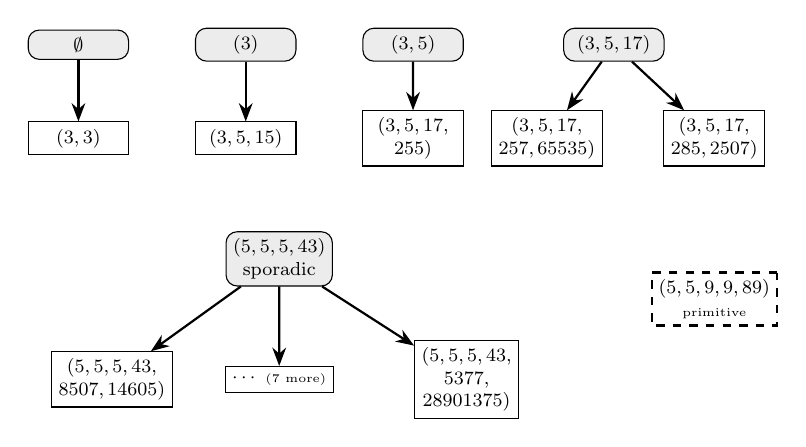
\begin{tikzpicture}[
  seed/.style={draw, rounded corners, fill=gray!15, minimum width=1.5cm,
    font=\footnotesize, align=center, inner sep=3pt},
  lehmer/.style={draw, fill=white, minimum width=1.5cm, font=\footnotesize,
    align=center, inner sep=3pt},
  arr/.style={-{Stealth}, thick},
  scale=0.85, transform shape
]
\node[seed] (s0) at (0,0) {$\emptyset$};
\node[lehmer] (l1) at (0,-1.4) {$(3,3)$};
\node[seed] (s1) at (2.5,0) {$(3)$};
\node[lehmer] (l2) at (2.5,-1.4) {$(3,5,15)$};
\node[seed] (s2) at (5,0) {$(3,5)$};
\node[lehmer] (l3) at (5,-1.4) {$(3,5,17,$\\$255)$};
\node[seed] (s3) at (8,0) {$(3,5,17)$};
\node[lehmer] (l4a) at (7,-1.4) {$(3,5,17,$\\$257,65535)$};
\node[lehmer] (l4b) at (9.5,-1.4) {$(3,5,17,$\\$285,2507)$};

\draw[arr] (s0) -- (l1);
\draw[arr] (s1) -- (l2);
\draw[arr] (s2) -- (l3);
\draw[arr] (s3) -- (l4a);
\draw[arr] (s3) -- (l4b);

\node[seed] (sp1) at (3,-3.2) {$(5,5,5,43)$\\sporadic};
\node[lehmer] (sp1a) at (0.5,-5) {$(5,5,5,43,$\\$8507,14605)$};
\node[lehmer] (sp1b) at (3,-5) {$\cdots$ {\tiny(7 more)}};
\node[lehmer] (sp1c) at (5.8,-5) {$(5,5,5,43,$\\$5377,$\\$28901375)$};
\draw[arr] (sp1) -- (sp1a);
\draw[arr] (sp1) -- (sp1b);
\draw[arr] (sp1) -- (sp1c);

\node[lehmer, dashed, thick] (prim) at (9.5,-3.8) {$(5,5,9,9,89)$\\
  {\tiny primitive}};
\end{tikzpicture}
\caption{A fragment of~$\mathcal{G}_2$.  Rounded: plus-seeds.
Solid: derived Lehmer factorizations.  Dashed: primitive.  The
$(5,5,5,43)$ subtree exhibits both children: the Lehmer descendant
$(5,5,5,43,5375)$ via $x = E$, and the chain extension
$(5,5,5,43,5377)$ via $x = E + 2$.}\label{fig:tree}
\end{figure}


%=====================================================================
\section{Partial results at $r = 8$}\label{sec:r8-partial}
%=====================================================================

A complete $r = 8$ census remains out of reach with the current
algorithm, even with the finishing-feasibility sharpening of
Section~\ref{sec:finishing}: the dominant cost is the search through
non-plus-seed length-$6$ prefixes, which is roughly three orders of
magnitude more expensive than the corresponding $r = 7$ search.
However, the chain theory of Section~\ref{sec:plus-seed-chains}
furnishes \emph{closed-form} enumerations of two canonical $r = 8$
subtrees, providing the first concrete $r = 8$ data.

\subsection{The Fermat-$6$ subtree}

By Theorem~\ref{thm:plus-seed-closure} applied to the Fermat-$6$
plus-seed $F^{(6)} = (3, 5, 17, 257, 65537, 4294967297)$, the
length-$8$ extensions are in bijection with divisor pairs of
$M_{F^{(6)}} = E^2 + E - 1 = 2^{128} - 2^{64} - 1$.  This integer
factors as
\[
  2^{128} - 2^{64} - 1
  \;=\;
  29 \cdot 101 \cdot 1061 \cdot 1741 \cdot p_{29},
\]
where $p_{29} = 62893522383172982457806872591$ is a $29$-digit prime,
giving $\tau(M_{F^{(6)}}) / 2 = 16$ length-$8$ Lehmer extensions.
The factorization completes in milliseconds via Pollard-rho ECM, so
the entire Fermat-$6$ subtree at $r = 8$ enumerates in well under one
second.

\subsection{The sporadic-$6$ subtree}

The sporadic chain rooted at $(5, 5, 5, 43)$ reaches length $6$ at
$S^{(6)} = (5, 5, 5, 43, 5377, 28901377)$.  By the same theorem, the
length-$8$ extensions of $S^{(6)}$ are governed by the divisors of
$M_{S^{(6)}} = E^2 + E - 1$ with $E = 5 \cdot 5 \cdot 5 \cdot 43
\cdot 5377 \cdot 28901377 \approx 8.35 \times 10^{14}$.  Direct
factorization of $M_{S^{(6)}} \approx 7.0 \times 10^{29}$ is feasible
in seconds.

More broadly, every length-$6$ plus-seed---including the six fresh
sporadic length-$6$ plus-seeds in Table~\ref{tab:chains}---contributes
$\tau(M)/2$ length-$8$ Lehmer extensions in closed form.

\subsection{What remains for a complete $r = 8$ census}

The closed-form subtrees account for plus-seed length-$6$ prefixes,
and the descent picture (Theorem~\ref{thm:descent-formula})
guarantees that any length-$8$ Lehmer factorization with descended
pair $(a, b)$ has a length-$6$ plus-seed parent.  Therefore the
\emph{derived} length-$8$ factorizations are exactly the union of
plus-seed closedness contributions over all length-$6$ plus-seeds.
What remains is to enumerate:
\begin{enumerate}[label=(\roman*)]
  \item all length-$6$ $k = 2$-plus-seeds (the chain forest at
    length $6$), and
  \item all \emph{primitive} length-$8$ $k = 2$ factorizations.
\end{enumerate}
Both items reduce to a length-$6$ plus-seed enumeration: by
Theorem~\ref{thm:chain-existence}, every length-$6$ plus-seed either
is a chain extension of a length-$5$ plus-seed (six known) or is
\emph{fresh} (a length-$5$ prefix that is not a plus-seed but
extends to a length-$6$ plus-seed via the closed equation
$x_6 = (B + 1)/A$ at the length-$5$ partial factorization).  The
fresh enumeration is not yet complete; we leave its determination
as the principal computational open problem at $r = 8$.


%=====================================================================
\section{Open questions}
%=====================================================================

\begin{enumerate}[label=\arabic*.]
  \item \textbf{Finiteness of primitives.}  All known truly-primitive
    $2$-Lehmer factorizations have $|G| \ge 5$.  Are there finitely many
    for each~$k$?

  \item \textbf{Realizability.}  Which spoof factorizations correspond
    to actual integers $n = p_1^{\alpha_1} \cdots p_r^{\alpha_r}$ with
    each $x_i = p_i^{\alpha_i}$ a prime power?

  \item \textbf{Fresh plus-seed growth.}  At lengths $4, 5, 6$ we
    observe $1, 4, 6$ fresh plus-seeds respectively (the length-$6$
    count via inverse parent inference; the true length-$6$ count may
    be higher).  Does the number of fresh plus-seeds at length $s$
    grow polynomially, exponentially, or remain bounded?

  \item \textbf{Density of primitives.}  Among the $103$ $k = 2$
    factorizations with $r \le 7$, $41$ are truly primitive
    ($\approx 40\%$).  Does this proportion converge?

  \item \textbf{Length-$6$ plus-seed enumeration.}  Direct enumeration
    of all length-$6$ plus-seeds (without going through the $r = 7$
    Lehmer census) would extend the $r = 8$ partial results of
    Section~\ref{sec:r8-partial} to a complete derived-factorization
    enumeration via Theorem~\ref{thm:plus-seed-closure}.

  \item \textbf{Sharper $u_{\max}$ bound.}  Both length-$4$ $k = 2$
    plus-seeds in our census exhibit $u_{\max} \approx 0.6 \cdot E$
    (Remark~\ref{rem:umax-empirical}), and spot-checks on three
    length-$5$ plus-seeds find no productive $u$ above $\sqrt{EB}$,
    while the provable bound is $u \le 2E + 1 \approx 2 \sqrt{EB}$.
    We conjecture the correct bound is $u^2 \le EB$ (equivalently
    $u \le \sqrt{E(E+1)}$) for every $k = 2$ plus-seed; a proof
    would likely require analyzing the divisor structure of $M_u =
    u^2 EB + uC + (EB)^2$ in the residue class $-EB \pmod u$ in the
    regime $u^2 > EB$, which the divisor-density heuristic does not
    capture.
\end{enumerate}


\appendix

%=====================================================================
\section{Full census listing (organized by chain forest)}\label{app:full-census}
%=====================================================================

The complete $r \le 7$, $k = 2$ census is presented below in
hierarchical form: each plus-seed appears as a section header
(annotated with its chain identification, depth in the chain, and
$\eps$ value), followed by its descended-pair and Lehmer-companion
children.  The chain ordering is Fermat first (depth $0$ to $5$), then
sporadic chains in the order they first appear in
Table~\ref{tab:chains}.  Descended children within a section are
sorted by the second-to-last factor $x_{r-1}$.  Truly primitive
factorizations (those with no plus-seed parent of either kind) appear
at the end, grouped by length.

% --- Table B: Lehmer factorizations grouped by parent plus-seed ---
% Requires \usepackage{longtable} in the preamble.
\begin{longtable}{@{}p{0.95\linewidth}@{}}
\caption{The $r \le 7$ $k = 2$-Lehmer factorizations grouped by
parent plus-seed.  Each plus-seed appears as a section header,
followed by its descended-pair and Lehmer-companion children.
Truly primitive factorizations (no plus-seed parent of either
kind) appear at the end.}\label{tab:census-organized}\\
\toprule
\endfirsthead
\multicolumn{1}{@{}l}{\textit{(continued from previous page)}}\\
\toprule
\endhead
\bottomrule
\multicolumn{1}{r@{}}{\textit{(continued on next page)}}\\
\endfoot
\bottomrule
\endlastfoot
\textbf{$(3)$} \quad (Fermat, depth 1, $\eps = 3$): \\
\quad $(3,\,5,\,15)$ \hfill {\small descended} \\
\addlinespace
\textbf{$(3,\,5)$} \quad (Fermat, depth 2, $\eps = 15$): \\
\quad $(3,\,5,\,17,\,255)$ \hfill {\small descended} \\
\addlinespace
\textbf{$(3,\,5,\,17)$} \quad (Fermat, depth 3, $\eps = 255$): \\
\quad $(3,\,5,\,17,\,257,\,65535)$ \hfill {\small descended} \\
\quad $(3,\,5,\,17,\,285,\,2507)$ \hfill {\small descended} \\
\addlinespace
\textbf{$(3,\,5,\,17,\,257)$} \quad (Fermat, depth 4, $\eps = 65535$): \\
\quad $(3,\,5,\,17,\,257,\,65537,\,4294967295)$ \hfill {\small descended} \\
\quad $(3,\,5,\,17,\,257,\,65555,\,226112997)$ \hfill {\small descended} \\
\quad $(3,\,5,\,17,\,257,\,65717,\,23794275)$ \hfill {\small descended} \\
\quad $(3,\,5,\,17,\,257,\,68975,\,1314417)$ \hfill {\small descended} \\
\addlinespace
\textbf{$(3,\,5,\,17,\,257,\,65537)$} \quad (Fermat, depth 5, $\eps = 4294967295$): \\
\quad $(3,\,5,\,17,\,257,\,65537,\,4294967297,\,18446744073709551615)$ \hfill {\small descended} \\
\quad $(3,\,5,\,17,\,257,\,65537,\,4294967307,\,1676976737878111325)$ \hfill {\small descended} \\
\quad $(3,\,5,\,17,\,257,\,65537,\,4294967367,\,259813301047285385)$ \hfill {\small descended} \\
\quad $(3,\,5,\,17,\,257,\,65537,\,4294967375,\,233503093781227857)$ \hfill {\small descended} \\
\quad $(3,\,5,\,17,\,257,\,65537,\,4294968077,\,23619394908814395)$ \hfill {\small descended} \\
\quad $(3,\,5,\,17,\,257,\,65537,\,4294968165,\,21227557884627347)$ \hfill {\small descended} \\
\quad $(3,\,5,\,17,\,257,\,65537,\,4294968305,\,18282208526299887)$ \hfill {\small descended} \\
\quad $(3,\,5,\,17,\,257,\,65537,\,4294972905,\,3288780203224487)$ \hfill {\small descended} \\
\quad $(3,\,5,\,17,\,257,\,65537,\,4294978395,\,1662022861452077)$ \hfill {\small descended} \\
\quad $(3,\,5,\,17,\,257,\,65537,\,4295028995,\,298983922990677)$ \hfill {\small descended} \\
\quad $(3,\,5,\,17,\,257,\,65537,\,4295038935,\,257500129211417)$ \hfill {\small descended} \\
\quad $(3,\,5,\,17,\,257,\,65537,\,4295047007,\,231424601693025)$ \hfill {\small descended} \\
\quad $(3,\,5,\,17,\,257,\,65537,\,4295755325,\,23413007171307)$ \hfill {\small descended} \\
\quad $(3,\,5,\,17,\,257,\,65537,\,4295844117,\,21042504669635)$ \hfill {\small descended} \\
\quad $(3,\,5,\,17,\,257,\,65537,\,4300626777,\,3263735907095)$ \hfill {\small descended} \\
\quad $(3,\,5,\,17,\,257,\,65537,\,4357221587,\,300607780005)$ \hfill {\small descended} \\
\addlinespace
\textbf{$(5,\,5,\,5,\,43)$} \quad (sporadic root, $\eps = 5375$): \\
\quad $(5,\,5,\,5,\,43,\,5375)$ \hfill {\small companion} \\
\quad $(5,\,5,\,5,\,43,\,5377,\,28901375)$ \hfill {\small descended} \\
\quad $(5,\,5,\,5,\,43,\,5387,\,2632285)$ \hfill {\small descended} \\
\quad $(5,\,5,\,5,\,43,\,5407,\,937505)$ \hfill {\small descended} \\
\quad $(5,\,5,\,5,\,43,\,5477,\,291475)$ \hfill {\small descended} \\
\quad $(5,\,5,\,5,\,43,\,5717,\,90115)$ \hfill {\small descended} \\
\quad $(5,\,5,\,5,\,43,\,6215,\,39817)$ \hfill {\small descended} \\
\quad $(5,\,5,\,5,\,43,\,6487,\,31385)$ \hfill {\small descended} \\
\quad $(5,\,5,\,5,\,43,\,8507,\,14605)$ \hfill {\small descended} \\
\addlinespace
\textbf{$(3,\,5,\,17,\,353,\,929)$} \quad (sporadic root, $\eps = 83623935$): \\
\quad $(3,\,5,\,17,\,353,\,929,\,83623935)$ \hfill {\small companion} \\
\quad $(3,\,5,\,17,\,353,\,929,\,83623937,\,6992962672132095)$ \hfill {\small descended} \\
\quad $(3,\,5,\,17,\,353,\,929,\,83623955,\,368050746176997)$ \hfill {\small descended} \\
\quad $(3,\,5,\,17,\,353,\,929,\,84866225,\,5712718767)$ \hfill {\small descended} \\
\quad $(3,\,5,\,17,\,353,\,929,\,107227427,\,379892085)$ \hfill {\small descended} \\
\addlinespace
\textbf{$(3,\,9,\,9,\,23,\,131)$} \quad (sporadic root, $\eps = 732159$): \\
\quad $(3,\,9,\,9,\,23,\,131,\,732159)$ \hfill {\small companion} \\
\quad $(3,\,9,\,9,\,23,\,131,\,732161,\,536058265599)$ \hfill {\small descended} \\
\addlinespace
\textbf{$(5,\,5,\,5,\,43,\,5377)$} \quad (sporadic, depth 1, $\eps = 28901375$): \\
\quad $(5,\,5,\,5,\,43,\,5377,\,28901377,\,835289534693375)$ \hfill {\small descended} \\
\addlinespace
\textbf{$(5,\,5,\,5,\,47,\,453)$} \quad (sporadic root, $\eps = 2661375$): \\
\quad $(5,\,5,\,5,\,47,\,453,\,2661375)$ \hfill {\small companion} \\
\quad $(5,\,5,\,5,\,47,\,453,\,2661377,\,7082922213375)$ \hfill {\small descended} \\
\quad $(5,\,5,\,5,\,47,\,453,\,2661587,\,33571000485)$ \hfill {\small descended} \\
\quad $(5,\,5,\,5,\,47,\,453,\,2662317,\,7529674715)$ \hfill {\small descended} \\
\quad $(5,\,5,\,5,\,47,\,453,\,2665797,\,1604769395)$ \hfill {\small descended} \\
\quad $(5,\,5,\,5,\,47,\,453,\,2669445,\,880455347)$ \hfill {\small descended} \\
\quad $(5,\,5,\,5,\,47,\,453,\,2859927,\,38334425)$ \hfill {\small descended} \\
\quad $(5,\,5,\,5,\,47,\,453,\,3594207,\,10254305)$ \hfill {\small descended} \\
\quad $(5,\,5,\,5,\,47,\,453,\,4363935,\,6821537)$ \hfill {\small descended} \\
\addlinespace
\textbf{$(5,\,7,\,7,\,7,\,133)$} \quad (sporadic root, $\eps = 228095$): \\
\quad $(5,\,7,\,7,\,7,\,133,\,228095)$ \hfill {\small companion} \\
\quad $(5,\,7,\,7,\,7,\,133,\,228097,\,52027785215)$ \hfill {\small descended} \\
\quad $(5,\,7,\,7,\,7,\,133,\,230447,\,22358065)$ \hfill {\small descended} \\
\quad $(5,\,7,\,7,\,7,\,133,\,232717,\,11487035)$ \hfill {\small descended} \\
\quad $(5,\,7,\,7,\,7,\,133,\,232885,\,11092067)$ \hfill {\small descended} \\
\addlinespace
\textbf{$(3,\,5,\,17,\,257,\,65729,\,22318913)$} \quad (sporadic root, $\eps = 96139834027933695$): \\
\quad $(3,\,5,\,17,\,257,\,65729,\,22318913,\,96139834027933695)$ \hfill {\small companion} \\
\addlinespace
\textbf{$(3,\,5,\,17,\,365,\,855,\,7234467)$} \quad (sporadic root, $\eps = 575712553701375$): \\
\quad $(3,\,5,\,17,\,365,\,855,\,7234467,\,575712553701375)$ \hfill {\small companion} \\
\addlinespace
\textbf{$(3,\,11,\,11,\,11,\,677,\,3659)$} \quad (sporadic root, $\eps = 9891231999$): \\
\quad $(3,\,11,\,11,\,11,\,677,\,3659,\,9891231999)$ \hfill {\small companion} \\
\addlinespace
\textbf{$(5,\,5,\,5,\,43,\,5413,\,786349)$} \quad (sporadic root, $\eps = 22878725861375$): \\
\quad $(5,\,5,\,5,\,43,\,5413,\,786349,\,22878725861375)$ \hfill {\small companion} \\
\addlinespace
\textbf{$(5,\,5,\,5,\,53,\,215,\,158265)$} \quad (sporadic root, $\eps = 225428709375$): \\
\quad $(5,\,5,\,5,\,53,\,215,\,158265,\,225428709375)$ \hfill {\small companion} \\
\addlinespace
\textbf{$(5,\,7,\,7,\,13,\,13,\,619)$} \quad (sporadic root, $\eps = 25629695$): \\
\quad $(5,\,7,\,7,\,13,\,13,\,619,\,25629695)$ \hfill {\small companion} \\
\addlinespace
\midrule
\textbf{Truly primitive factorizations (no plus-seed parent)}: \\
\quad $(5,\,5,\,9,\,9,\,89)$ \hfill {\small $r = 5$} \\
\quad $(3,\,5,\,17,\,377,\,1217,\,2295)$ \hfill {\small $r = 6$} \\
\quad $(3,\,5,\,17,\,395,\,1059,\,2303)$ \hfill {\small $r = 6$} \\
\quad $(3,\,5,\,33,\,53,\,69,\,8343)$ \hfill {\small $r = 6$} \\
\quad $(5,\,5,\,5,\,45,\,807,\,267023)$ \hfill {\small $r = 6$} \\
\quad $(5,\,5,\,5,\,47,\,457,\,50659)$ \hfill {\small $r = 6$} \\
\quad $(5,\,5,\,5,\,65,\,129,\,2325)$ \hfill {\small $r = 6$} \\
\quad $(3,\,5,\,17,\,257,\,65543,\,613622973,\,8815156799949437)$ \hfill {\small $r = 7$} \\
\quad $(3,\,5,\,17,\,257,\,65543,\,613627757,\,78010845360333)$ \hfill {\small $r = 7$} \\
\quad $(3,\,5,\,17,\,257,\,65555,\,226113003,\,8596590110981999)$ \hfill {\small $r = 7$} \\
\quad $(3,\,5,\,17,\,257,\,65583,\,91446429,\,1862725578762405)$ \hfill {\small $r = 7$} \\
\quad $(3,\,5,\,17,\,257,\,65855,\,14660375,\,175338855)$ \hfill {\small $r = 7$} \\
\quad $(3,\,5,\,17,\,257,\,66023,\,8884637,\,90028574052093)$ \hfill {\small $r = 7$} \\
\quad $(3,\,5,\,17,\,257,\,66035,\,12360093,\,29069129)$ \hfill {\small $r = 7$} \\
\quad $(3,\,5,\,17,\,257,\,66527,\,4399443,\,249102573029243)$ \hfill {\small $r = 7$} \\
\quad $(3,\,5,\,17,\,257,\,70953,\,1015619,\,5544845)$ \hfill {\small $r = 7$} \\
\quad $(3,\,5,\,17,\,257,\,72113,\,719417,\,599253543)$ \hfill {\small $r = 7$} \\
\quad $(3,\,5,\,17,\,257,\,72939,\,645693,\,6040018747905)$ \hfill {\small $r = 7$} \\
\quad $(3,\,5,\,17,\,257,\,75273,\,506627,\,1912164594413)$ \hfill {\small $r = 7$} \\
\quad $(3,\,5,\,17,\,257,\,85185,\,288275,\,19698725)$ \hfill {\small $r = 7$} \\
\quad $(3,\,5,\,17,\,257,\,103943,\,199577,\,1593393)$ \hfill {\small $r = 7$} \\
\quad $(3,\,5,\,17,\,257,\,104093,\,176927,\,1175218174293)$ \hfill {\small $r = 7$} \\
\quad $(3,\,5,\,17,\,263,\,9585,\,27948617,\,125635487981969)$ \hfill {\small $r = 7$} \\
\quad $(3,\,5,\,17,\,263,\,11159,\,78249,\,506759)$ \hfill {\small $r = 7$} \\
\quad $(3,\,5,\,17,\,269,\,5279,\,19059029,\,809372846673)$ \hfill {\small $r = 7$} \\
\quad $(3,\,5,\,17,\,269,\,5283,\,5104049,\,80419259566169)$ \hfill {\small $r = 7$} \\
\quad $(3,\,5,\,17,\,287,\,2363,\,4762259,\,252056385)$ \hfill {\small $r = 7$} \\
\quad $(3,\,5,\,17,\,363,\,887,\,36705,\,1780076619)$ \hfill {\small $r = 7$} \\
\quad $(3,\,5,\,17,\,387,\,755,\,837215,\,12806102345)$ \hfill {\small $r = 7$} \\
\quad $(3,\,5,\,17,\,419,\,659,\,172587,\,68725637)$ \hfill {\small $r = 7$} \\
\quad $(3,\,5,\,23,\,95,\,207,\,215,\,85803023)$ \hfill {\small $r = 7$} \\
\quad $(3,\,5,\,27,\,45,\,233,\,42489,\,1389617)$ \hfill {\small $r = 7$} \\
\quad $(3,\,5,\,33,\,33,\,359,\,4869,\,2502245)$ \hfill {\small $r = 7$} \\
\quad $(5,\,5,\,5,\,43,\,5479,\,327773,\,2239165)$ \hfill {\small $r = 7$} \\
\quad $(5,\,5,\,5,\,43,\,5603,\,132673,\,9536030197)$ \hfill {\small $r = 7$} \\
\quad $(5,\,5,\,5,\,43,\,5623,\,122489,\,119765185)$ \hfill {\small $r = 7$} \\
\quad $(5,\,5,\,5,\,43,\,5759,\,80825,\,2587288073)$ \hfill {\small $r = 7$} \\
\quad $(5,\,5,\,5,\,43,\,6985,\,23335,\,28261225505)$ \hfill {\small $r = 7$} \\
\quad $(5,\,5,\,5,\,43,\,8749,\,13943,\,1335400765)$ \hfill {\small $r = 7$} \\
\quad $(5,\,5,\,5,\,47,\,535,\,2947,\,36041983)$ \hfill {\small $r = 7$} \\
\quad $(5,\,5,\,5,\,49,\,355,\,3619,\,183001469)$ \hfill {\small $r = 7$} \\
\end{longtable}


\begin{thebibliography}{9}

\bibitem{H26}
E.~Hasanalizade, \emph{Some remarks on a paper of Molnar and Singh},
Integers \textbf{26} (2026).

\bibitem{L32}
D.~H.~Lehmer, \emph{On Euler's totient function}, Bull.\ Amer.\ Math.\
Soc.\ \textbf{38} (1932), 745--751.

\bibitem{MS26}
G.~Molnar and G.~Singh, \emph{Spoof Lehmer factorizations}, Integers
\textbf{26} (2026), \#A33.

\bibitem{N15}
P.~Nielsen, \emph{Odd perfect numbers, Diophantine equations, and upper
bounds}, Math.\ Comp.\ \textbf{84} (2015), 2549--2567.

\bibitem{sympy}
A.~Meurer et al., \emph{SymPy: symbolic computing in Python}, PeerJ
Computer Science \textbf{3} (2017), e103.

\end{thebibliography}

\end{document}
